\documentclass[13pt, a4paper, twoside]{article}
\usepackage[utf8]{inputenc}
\usepackage{geometry}
\usepackage[czech]{babel}
\usepackage{chemformula}
\usepackage{chemfig}
\usepackage{enumitem}
\usepackage{fancyhdr}
\usepackage{float}
\usepackage{setspace}
\usepackage{multicol}
\geometry{legalpaper, margin=1.05in}
\pagestyle{fancy}
\lhead{\Large Šárka Doležalová, skupina 6}
\rhead{\large 10.12.2020}
\begin{document}
\begin{center}
    \Huge
    Úloha 3: Identifikace a stanovení koncentrace organické kyseliny
\end{center}
\large
\onehalfspacing
\section*{Zadané Úlohy}
\begin{enumerate}
    \item Připravte zásobní roztok hydroxidu sodného a pomocí titrace primárního standardu –
    dihydrátu kyseliny šťavelové – stanovte jeho přesnou koncentraci.
    \item Pomocí acidobazické titrace s vizuální detekcí bodu ekvivalence stanovte celkovou
    koncentraci protonů v roztoku neznámé organické kyseliny.
    \item Pomocí potenciometrické titrace stanovte disociační konstantu pKA1 nebo pKA2 předložené
    organické kyseliny. Podle zjištěné hodnoty pKA identifikujte, jaká kyselina je přítomna ve
    vzorku, a určete její koncentraci.
\end{enumerate}
\section*{Teoretický úvod}
    \subsection*{Práce s pH-metrem}
        Pro změření pH, které je chápáno jako záporný dekadický logaritmus koncentrace
        oxoniových kationů, využíváme pH-metru. Toto zřízení je citlivý voltmetr. Ten
        na svých elektrodách (v našem případě je používána sklěněná kombinovaná elektroda)
        měří změnu napětí.
    \subsection*{Acidobazická titrace}
    Tato metoda určuje množství báze přítomné ve vzorku pomocí titrace odměrným roztokem
    kyseliny (acidimetrie), nbeo množství kyseliny ve vzorku pomocí titrace odměrným
    roztokem báze (alkilimetrie). Acidobazický indikátor je látka, jež při vstyku se vzorek
    během titrace protonizuje, či deprotonizuje (chová se jako kyselina, nebo báze), přičemž
    změní barvu. Při titraci je směs neustále míchána v titrační baňce krouživými pohyby
    za pozvolného přidávání titračního činidla z byrety.
    
    V našem případě je určována koncentrace neznámé
    organické kyseliny. Jako acidobazický indikátor je využit fenoloftalein, jedná se
    tedy o alkilimetrii.
    \subsection*{Stanovení přesné koncetrace zásobního roztoku}
    Při záměru stanovení přesné koncentrace zásobního roztoku je potřeba využít titrace
    primárního standardu. Primární standard je látka, která je relativně stálá a čistá
    a má především dobře definované složení.

    \section*{Postup}
    \subsection*{Příprava odměrného roztoku hydroxidu sodného}
    Bylo připraveno 250 ml roztou NaOH o koncentraci c=0,1 mol/dm3
    (Bylo naváženo 1,00 g NaOH), poté odlito do odměrné baňky a zazátkováno.
    Obsah byl důkladně promíchán.
    \subsection*{Stanovení přesné koncentrace odměrného roztoku hydroxidu}
    Bylo odváženo $m_1$=0,0999 g kyseliny šťavelové ($M_1$ = 126,07 $g \cdot mol^{-1}$). Ta byla poté důkladně převedena (vymytím lodičky) do titrační baňky, kde byla rozpuštěna v 50 ml destilované vody. Poté bylo přidáno pár kapek fenolftaleinu.
    Odměrným roztokem hydroxidu byla naplněna byreta. Hladina roztoku byla zarovnána na nulu. Roztok kyseliny šťavelové byl titrován až do vzniku trvalého fialového zbarvení. Celý proces byl zopakován třikrát.
    
    \subsection*{Stanovení celkové koncentrace protonů v roztoku neznámé organické kyseliny}
    Z neznámé kyseliny bylo odpipetováno 20 ml, vzorek byl naředěn 30 ml destilované vody a bylo přidáno několik kapek fenolftaleinu. Tento roztek byl dále titrován roztokem NaOH, opět do začátku odbarvení. Postup byl opět třikrát zopakován.

    \subsection*{Kalibrace pH-metru}
    Očištěná elektroda byla ponořena do neutrálního pufru o známé hodnotě pH a poté byl nastaven konstantní činitel závislosti pH na napětí, tak aby se na displeji zobrazila daná hodnota pH. Elektroda byla očištěna a proces byl zopakován na kyselém pufru. Proces byl znovu zopakován s neutrálním pufrem.

    \subsection*{Stanovení disociační konstanty a identifikace neznámé organické kyseliny}
    Bylo odpipetováno 20 ml neznámé kyseliny, která byla zředěna 10 ml destilované vody. Do roztoku bylo vloženo magnetické míchadlo a kádinka byla postavena na magnetickou míchačku. Elektroda pH-metru byla položena do roztoku. Bylo zapsáno výchozí pH. Poté bylo přidáváno po 1,00 ml NaOH a vždy bylo zapsáno dané pH. Takto bylo postupováno až do přidání NaOH o objemu o 5,00 ml menší než objem NaOH pro neutralizaci při předchozí titraci. Déle byla +-5 ml od bodu ekvivalence přidávána NaOH po 0,50 ml a opět byla zapisována změna pH. Poté byl roztok NaOH opět přidáván po 1,00 ml až do převýšení ekvivalence o 15,00 ml. Z těchto údajů byla načrtnuta titrační křivka, podle ní bylo zjištěno že je kyselina jednosytná. Dále bylo určeno Pka kyseliny z prostřední spotřeby k ekvivalenci. Podle toho byla určena neznámá kyselina.
    
    \section*{Výpočty}
    \subsection*{Měření pH při titrování neznámé kyseliny}
    \begin{align*}
    pH &= \frac{1}{2}(pK_a - log(c_{H^+}))\\
    pK_a &= 2pH + log(c_{H^+})\\
    pK_a &= 4.49
    \end{align*}
    \section*{Tabulky}
    \subsection*{Tab. 1. - Titrace kyseliny šťavelové}
    \begin{figure}[H]
        \centering
        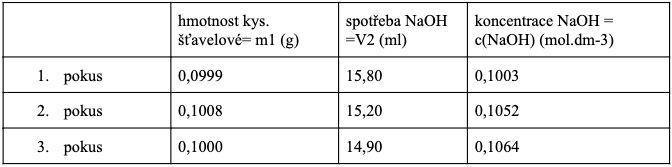
\includegraphics[width=7in]{kys_stav.png} 
    \end{figure}

    \begin{align*}
        c_{NaOH}=2\frac{m_1}{M_1 \cdot V_2}
    \end{align*}

    \subsection*{Tab. 2 - Titrace neznámé kyseliny}
    \begin{figure}[H]
        \centering
        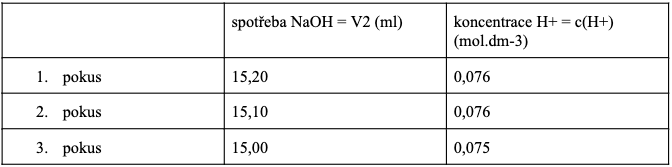
\includegraphics[width=7in]{kys_nez.png}
    \end{figure}
    \begin{align*}
        c_{H^+}=\frac{c_{NaOH}\cdot V_2}{V_1}
    \end{align*}
    \section*{Graf titrační křivky}
    \begin{figure}[H]
        \centering
        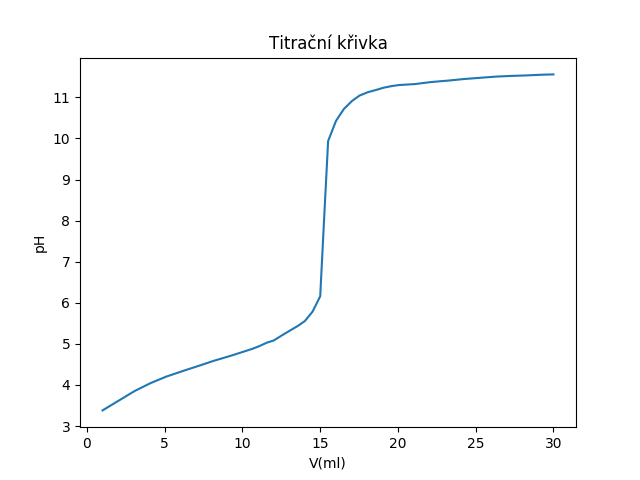
\includegraphics[width=5in]{titracni_krivka.png}
    \end{figure}

    \section*{Závěr}
    Hodnota $p_{KA}$ nám vyšla 4,49, což odpovídá mezi kyselinu benzoovou a octovou. Provedli jsme čichovou zkoušku a určili tak, že kyselina byla octová. Chyba pravděpodobně vznikla nedostačně přesným titrování.


\end{document}